%% LyX 2.2.3 created this file.  For more info, see http://www.lyx.org/.
%% Do not edit unless you really know what you are doing.
\documentclass[english]{article}
\usepackage[T1]{fontenc}
\usepackage[latin9]{inputenc}
\usepackage{babel}
\usepackage{float}
\usepackage{textcomp}
\usepackage{graphicx}
\usepackage[unicode=true,pdfusetitle,
 bookmarks=true,bookmarksnumbered=false,bookmarksopen=false,
 breaklinks=false,pdfborder={0 0 1},backref=false,colorlinks=false]
 {hyperref}

\makeatletter

%%%%%%%%%%%%%%%%%%%%%%%%%%%%%% LyX specific LaTeX commands.
%% Because html converters don't know tabularnewline
\providecommand{\tabularnewline}{\\}

\makeatother

\usepackage{listings}
\renewcommand{\lstlistingname}{Listing}

\begin{document}
\noindent \begin{center}
\includegraphics[scale=0.15]{\string"images/GitHub Banner\string".png}
\par\end{center}
\begin{quote}
\begin{center}
{\Huge{}Travlendar+}
\par\end{center}{\Huge \par}
\begin{center}
{\Large{}Design Document}
\par\end{center}{\Large \par}
\begin{center}
Calzavara Filippo, Filaferro Giovanni, Benedetto Maria Nespoli
\par\end{center}

\end{quote}
\begin{center}
Version 1.0.0
\par\end{center}

\bigskip{}
\noindent \begin{center}
\includegraphics[width=3cm]{images/PolimiLogo}
\par\end{center}

\pagebreak{}\tableofcontents{}

\pagebreak{}

\section{Introduction}

\subsection{Purpose}

The Design Document (DD) contains a functional description of ``Travlendar+'''s
System.

This document explains each component that will be inserted into the
system, its architecture and the design patterns that will be implemented
to ensure that all the requirements are satisfied.

Components will be described both at High Level and more in depth,
illustrating and explaining all the subcomponents every component
is made of.

The reader of this document will get a clear idea about its architecture
(hardware and software) whether he wants to have a detailed description
of the system or a more general one.

\subsection{Scope}

To learn about the Scope of the project look to the ``1.2 Scope''
section of the RASD document.

\subsection{Definitions, Acronyms, Abbreviations}

\subsubsection{Definitions}

\begin{tabular}{|c|c|}
\hline 
Definition & Explanation\tabularnewline
\hline 
\hline 
Appointment & A period of time in which something take place at a certain time\tabularnewline
\hline 
Travlendar+ & The name of the platform to develop\tabularnewline
\hline 
Event & A synonym for appointment \tabularnewline
\hline 
System & A synonym of Travlendar+\tabularnewline
\hline 
Up Coming Event & A particular event that is expected to occur soon\tabularnewline
\hline 
Up Next Event & A synonym of Up Coming\tabularnewline
\hline 
User & A potential utilizer of this project\tabularnewline
\hline 
Ride & A service performed by a ride-sharing company and Cabs\tabularnewline
\hline 
Mockup & A scale or full-size model of a design or device\tabularnewline
\hline 
RESTful API & API that follow the REST paradigm\tabularnewline
\hline 
Direction API & The name of Google Maps\texttrademark{} API service\tabularnewline
\hline 
\end{tabular}

\subsubsection{Acronyms}

\begin{tabular}{|c|c|}
\hline 
Acronym & Explanation\tabularnewline
\hline 
\hline 
GUI & Graphic User Interface\tabularnewline
\hline 
ETA & Estimated time of arrival\tabularnewline
\hline 
API & Application programming interface\tabularnewline
\hline 
RASD & Requirement Analysis and Specification Document\tabularnewline
\hline 
PNR & Passenger name record\tabularnewline
\hline 
QR & Quick Response Code\tabularnewline
\hline 
OS & Operative System\tabularnewline
\hline 
JSON & JavaScript Object Notation\tabularnewline
\hline 
REST & Representational State Transfer\tabularnewline
\hline 
APNS & Apple Push Notification Service\tabularnewline
\hline 
CRUD & Create, Read, Update, Delete\tabularnewline
\hline 
ER & Entity Relationship\tabularnewline
\hline 
TDD & Test Driven Development\tabularnewline
\hline 
\end{tabular}

\subsubsection{Abbreviations}

\begin{tabular}{|c|c|}
\hline 
Abbreviation & Explanation\tabularnewline
\hline 
\hline 
App & A synonym of Travlendar+\tabularnewline
\hline 
{[}Gn{]} & N-goal\tabularnewline
\hline 
{[}Dn{]} & N-domain assumption\tabularnewline
\hline 
{[}Rn{]} & N-functional requirement\tabularnewline
\hline 
\end{tabular}

\subsection{Revision History}
\begin{itemize}
\item 1.0.0 - Initial Version (13/11/2017) 
\end{itemize}

\subsection{Reference Documents}
\begin{itemize}
\item RASD document previously delivered.
\end{itemize}

\subsection{Document Structure}

The paper includes eight areas. The first one, is composed by the
introductory information provided in order to give an orientative
view of what this document is about. 

The second one provides an in-depth description of each Architectural
Design aspect which reflects the decisions that the team made.

The third section is about the algorithms that are designed to make
the full system work.

Then a ``User Interface Design'' section will go through the design
decisions.

Section five provides informations about how the requirements defined
in the RASD document map to the design elements defined in this document.

The sixth section will identify the order in which the subcomponents
of the system will be implemented and tested.

Finally, a seventh and a eight section allows the reader to learn
the effort spent on this project by each team member and the references
made in the whole paper.

\pagebreak{}

\section{Architectural Design}

Figure \ref{fig:General-tier} represents Travlendar+'s architecture,
based on a two physical tiers system with distributed application
and data. In order to maintain higher standard in terms of offline
reliability, the client application is provided of a presentation
level, application logic and data management that merely synchronizes
and fetch updates from the server through a non-faulty connection.
\begin{center}
\begin{figure}[H]
\begin{centering}
\includegraphics[scale=0.5]{images/tier}
\par\end{centering}
\caption{\label{fig:General-tier}General tier architecture for Travlendar+.
An application logic and data management layer is provided to the
client application for offline reliability}
\end{figure}
\par\end{center}

Nevertheless, most of the computation burden such as the scheduling,
is performed sever-side.

\pagebreak{}

The following subsections are presented as follows:
\begin{enumerate}
\item The first section, \emph{High-level components overview and their
interaction}, contains details on how the communication works and
how the server is structured
\item The second section describes the components of the application logic,
including the external services called via API and the ER diagram
\item The \emph{Deployment view} section contain a diagram with the interactions
between several components
\item The \emph{Runtime view }chapter includes more detailed sequence diagram
of most important interaction with the system
\item \emph{Component interfaces} section contains information regarding
the interface to be built in order to make intelligible different
system
\item Section \emph{Selected architectural styles and patterns} contains
the major settings of the implementation of the system 
\item Finally, a chapter named \emph{Other design decisions} describes further
decision detail taken into account during the developing of this document
\end{enumerate}
\pagebreak{}

\subsection{High-level components overview and their interaction}

The mobile application located on the client's phone connects to the
central server by sending REST Api calls in asynchronous mode with
a separated thread. The main server replies back with the information
requested using the JSON encoding, which is reinterpreted locally
by the application. An example of this interaction is reported on
Figure \ref{fig:General-architecture}.
\begin{center}
\begin{figure}[H]
\begin{centering}
\includegraphics[scale=0.5]{images/application}
\par\end{centering}
\caption{\label{fig:General-architecture}General architecture}
\end{figure}
\par\end{center}

The engineering team of this project has identified Heroku\texttrademark{}
Cloud as the most suitable platform to host the main server due its
performance and scalability features. As shown in Figure \ref{fig:Central-Server-Representation},
a centralized server is composed by three entities: the web server,
the application logic and the database. The first is in charge of
dealing with all HTTP/HTTPS API requests in a consistent and systematic
way. It also communicates with the application logic, which is the
second layer, also called Mobile App Services as it contains the logic
to run the computation. Finally, the last layer is the database which
stores the dataset making it available to the application logic. 
\begin{center}
\begin{figure}[H]
\begin{centering}
\includegraphics[scale=0.5]{images/heroku}
\par\end{centering}
\caption{\label{fig:Central-Server-Representation}Central Server relies on
Heroku Cloud. Its representation includes three layer connected to
each other }
\end{figure}
\par\end{center}

All three active parts hereinbefore described are could be located
into several machines: replication and load balancing issues are transparent
services provided by the Heroku platform

\subsection{Component view}

A high level component view and related interfaces are represented
at Figure \ref{fig:The-main-component}. The system is composed of
a major component, namely the \emph{Mobile Application}, that interacts
with two subsystems, \emph{Scheduling Services} and \emph{User Services}.
\begin{figure}[H]
\begin{centering}
\includegraphics[scale=0.4]{images/component-1}
\par\end{centering}
\caption{\label{fig:The-main-component}The high level component view of the
system}
\end{figure}
Each module that compose the subsystems is interfaced with the DataBase
(specifically the DBMS) in order to let each part work independently
and simultaneously.

\subsubsection{Component view of the Scheduling Services}
\begin{center}
\begin{figure}[H]
\begin{centering}
\includegraphics[scale=0.4]{images/component-2}
\par\end{centering}
\caption{The Scheduling Services: includes details on }
\end{figure}
\par\end{center}

The \emph{Calendar Module} works as calendar manager and offers the
methods to edit, add and remove calendar. It is its responsibility
to check calendar constrains such as duplicates. The \emph{Event Manager}
module allows the creation and managing of the events and handles
the rescheduling when necessary (see section \ref{subsec:Event-Schedule-Algorithm}
for more details). It also offers the interface that allows to fetch
information about previous events. This module is connected to Google
Maps API, Weather API provided by OpenWeatherMap and to Apple Push
Notification Server, that handles the notification system towards
the mobile application.

\subsubsection{Component view of the User Services}
\begin{center}
\begin{figure}[H]
\begin{centering}
\includegraphics[scale=0.4]{images/component-3}
\par\end{centering}
\caption{User Services in detail}
\end{figure}
\par\end{center}

User services contains an \emph{Account Manager Module} that handles
the login/auto-login functions (cf. Section 3.2.1 RASD document).
The \emph{Tickets module} provide tools to store the ticket provided
by the local transit company into the database. Moreover, a setting
module provides tools for setting managing such as the eco-friendly
mode or the external services available.

\pagebreak{}

\subsubsection{Entity relationship diagram}

The following diagram provides a graphical representation of the Database
Schema that will be adopted by the system

\begin{figure}[H]
\begin{centering}
\includegraphics[scale=0.35]{images/er}
\par\end{centering}
\caption{\label{fig:ER-Diagram}ER Diagram of the database}
\end{figure}

Further clarification regarding the schema:
\begin{itemize}
\item The column \emph{transports} is of type BIT(5) for simplicity. If
the bit is 1, the corresponding mean of transportation is enabled
for that event. From the leftmost to the rightmost bit, there are:
Walking, Biking, Public Transport, Sharing Services and Car.
\item The column \emph{repetitions} is of type BIT(7) for simplicity. If
the bit is 1, the event will repeat for the corresponding day of the
week. The leftmost bit is for Monday, and the rightmost is for Sunday.
\item The other BITs are BIT(1) meaning TRUE for 1 and FALSE for 0.
\end{itemize}

\subsection{Deployment view}
\begin{center}
\begin{figure}[H]
\begin{centering}
\hspace*{-1.0cm}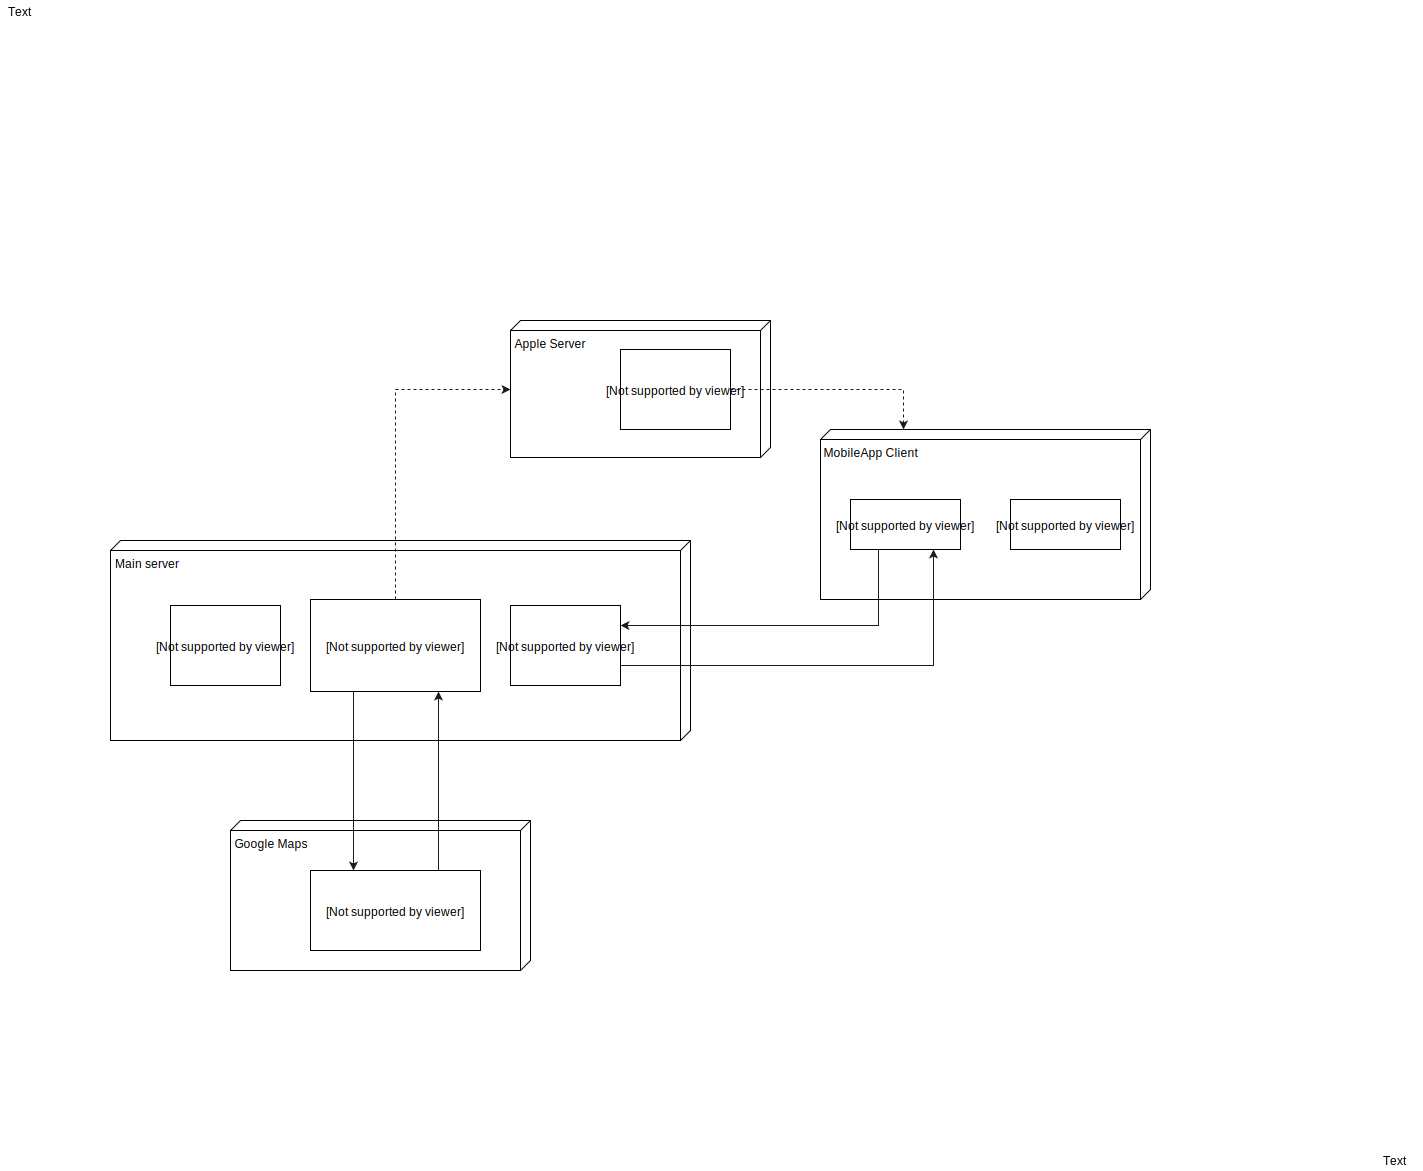
\includegraphics[scale=0.4]{images/highLevelComponent}
\par\end{centering}
\caption{\label{fig:High-level-components}High level components}
\end{figure}
\par\end{center}

\subsection{Runtime view}


\subsubsection{Create Calendar}

\hspace*{-3.5cm}\includegraphics[scale=0.5]{images/CreateCalendar}

\subsubsection{Add event}

\vspace*{-4cm}\hspace*{-0.5cm}\includegraphics[angle=90,scale=0.4]{images/AddStandardOrFlexibleEvent}

\subsubsection{Edit Preferences}

\includegraphics[angle=90,scale=0.4]{images/EditPreferences}

\subsubsection{Buy Ticket}

\hspace*{-3.0cm}\includegraphics[scale=0.4]{images/buyTicket}

\pagebreak{}

\subsection{Component interfaces}

In this section are described the interfaces that the Clients and
the Server will use in order to communicate

\subsubsection{RESTful API}

Our tiers will be connected through a network that will use a JSON
RESTful Application Programming Interface.

The API will lie on a Web server and will be called on a HTTP channel
with a classic TLS encryption layer

All the methods will require an authentication, except for the login
one. The exposed methods are:
\begin{itemize}
\item \textbf{/api/v1/login}
\begin{itemize}
\item POST: Allow the user to get an authentication token. If the user is
not present on the server database, he/she will be registered
\begin{itemize}
\item Parameters: \textbf{user\_token} A user token that is generated client
side by the application
\item Return: \textbf{device\_token} A token that will be used for future
authentication on that device with other APIs
\end{itemize}
\end{itemize}
\item \textbf{/api/v1/pushNotification}
\begin{itemize}
\item POST: Update the current push notification
\end{itemize}
\item \textbf{/api/v1/settings}
\begin{itemize}
\item GET: Retrieve the user settings
\item POST: Save some settings
\end{itemize}
\item \textbf{/api/v1/calendars}
\begin{itemize}
\item GET: Retrieve the user calendars
\item POST: Save some calendars
\end{itemize}
\item \textbf{/api/v1/events}
\begin{itemize}
\item GET: Retrieve the user events
\item POST: Save some events
\end{itemize}
\item \textbf{/api/v1/schedule}
\begin{itemize}
\item GET: Retrieve the user schedule
\end{itemize}
\item \textbf{/api/v1/position}
\begin{itemize}
\item POST: Update the current user position
\end{itemize}
\end{itemize}

\subsection{Selected architectural styles and patterns}

\subsubsection{Overall Architecture}

Our system will be composed of two tiers:
\begin{enumerate}
\item A client executable, that will run on an iOS device
\item A server part, that will be served on a scalable Heroku instance
\end{enumerate}
Each part will need a database: the server will store any piece of
information about users, calendars and events on its database, while
the client's database will have a cached copy of some events and calendars.

\subsubsection{Data Definition Language}

The following DDL in a SQL-like language is proposed for the database

\begin{figure}[H]
\begin{centering}
\vspace*{-2cm}\includegraphics[scale=0.4]{images/DDL}
\par\end{centering}
\caption{DDL}

\end{figure}

\subsubsection{Design Pattern}
\begin{itemize}
\item \textbf{Client-Server}: This is the most useful and common pattern,
that allow us to process the data acquisition and elaboration separately
from the client logic. Moreover, using this pattern we can create
simpler clients, and make the system more scalable: in fact, in order
to scale the entire system, we can simply add more server, and keep
the client the same.
\item \textbf{Singleton}: Server-side the server app will be a Singleton,
while client side there will be a API Manager as Singleton
\item \textbf{Publish/Subscribe}: Used for the push notifications between
the clients and the server
\end{itemize}

\subsection{Other design decisions}

We'll also use an external map service and a Weather API service,
in order to find the best travel route, and to show to the user the
events in a map view according to the weather forecast. To achieve
this aim, we'll use the Google Maps Directions API and OpenWeatherMap.

\pagebreak{}

\section{Algorithm Design}

In this section will be presented a description and an example code
of the main algorithms for the Travlendar+ platform.

Code provided in these subsections will be written in C++ or pseudo-code
that uses its syntax in order to better understand it without making
the reading too complex.

Functions that will be called and not specified in each Subsection
can be found in Subsection \ref{subsec:Other-Functions}.

\subsection{\label{subsec:Event-Schedule-Algorithm}Event Schedule Algorithm}

\subsubsection{Description}

This algorithm is the one who takes all users's events and tries to
schedule them whether possible according to user preferences and distance
from places. This will run Server Side.

Such function prepares a schedule following these steps:
\begin{enumerate}
\item Builds an array of events for each calendar of the given user;
\item Filters those events and divided them in two arrays of fixed and flexible
events as described in Subsection \ref{subsec:Flexible-Event-Fitting-Order-Algorythm};
\item It tries to fit them in the schedule:
\begin{enumerate}
\item If it succeeds (they are fittable and reachable) it adds them to the
fixed array and considers them as fixed;
\item If it fails, it sends a notification to the user;
\end{enumerate}
\item Then it tries to check if the other fixed events are reachable using
the reachability function described in Subsection \ref{subsec:Reachability-Function};
\item It terminates returning the created schedule.
\end{enumerate}

\paragraph{Main Function:}

\begin{lstlisting}[language={C++},basicstyle={\small\rmfamily},breaklines=true]
Schedule* schedule(
	User *u, 
	unsigned long date1, 
	unsigned long date2
);
\end{lstlisting}

This is the main one that takes in:
\begin{itemize}
\item \textbf{u}: user reference;
\item \textbf{date1}: start date;
\item \textbf{date2}: ending date.
\end{itemize}

\paragraph{Overloaded Functions:}

\subparagraph{Overload 1:}

Schedule function that checks just the 12 hours before and after the
event as parameter that has been created, modified or deleted.

\begin{lstlisting}[language={C++},basicstyle={\small\rmfamily},breaklines=true]
Schedule* schedule(
	User *u,
	Event *e
);
\end{lstlisting}

This is the first one overloaded that takes in:
\begin{itemize}
\item \textbf{u}: user reference;
\item \textbf{e}: event needing reschedule;
\end{itemize}

\subparagraph{Overload 2:}

Schedule function that checks the next hours, this can be called when
user uploads his current position or the system calls it every 2 hours;

\begin{lstlisting}[language={C++},basicstyle={\small\rmfamily},breaklines=true]
Schedule* schedule(User *u);
\end{lstlisting}

This is the first one overloaded that takes in:
\begin{itemize}
\item \textbf{u}: user reference;
\end{itemize}

\subsubsection{Example of Implementation}

Overloads:
\begin{center}
\includegraphics[scale=0.4]{images/code/s_overload}
\par\end{center}

Main Function:
\begin{center}
\includegraphics[scale=0.6]{images/code/s__1}
\par\end{center}

\begin{center}
\includegraphics[scale=0.6]{images/code/s__2}
\par\end{center}

\begin{center}
\includegraphics[scale=0.6]{images/code/s__3}
\par\end{center}

\begin{center}
\includegraphics[scale=0.6]{images/code/s__4}
\par\end{center}

\subsection{\label{subsec:Flexible-Event-Fitting-Order-Algorythm}Flexible Event
Fitting Order Algorithm}

\subsubsection{Description}

This is the algorithm that will be triggered when section \ref{subsec:Event-Schedule-Algorithm}'s
functions calls:
\begin{lstlisting}[language={C++},basicstyle={\small\rmfamily},breaklines=true]
void filterEvents(
	vector<Event> *main,
	vector<Event> *fixed,
	vector<Event> *flexible
);
\end{lstlisting}

Such function will do the following:
\begin{enumerate}
\item Put fixed events contained in \textbf{main} to \textbf{fixed} vector
and sort them by happening date;
\item Put flexible events contained in \textbf{main} to \textbf{flexible}
vector;
\item Sort \textbf{flexible} vector using the fitness function described
above.
\end{enumerate}
\begin{figure}[H]
\[
fittability(e)=1-\frac{duration(e)}{end(e)-start(e)-occupiedRange(c)}
\]

\caption{\label{fig:Fittability-Function}Fittability Function}
\end{figure}

This mathematical function takes into:
\begin{itemize}
\item \textbf{duration}(e): the duration of the flexible event;
\item \textbf{end}(e): preferred end time interval of flexible event;
\item \textbf{start}(e): preferred start time interval of flexible event;
\item \textbf{occupiedRange}(c): number of hours already occupied in that
range by other events in the event's calendar.
\end{itemize}

\subsubsection{Example of Implementation}
\begin{center}
\includegraphics[scale=0.6]{images/code/fitting}
\par\end{center}

This piece of code uses also this utility function in order to get
the fitness value of an event:
\begin{center}
\includegraphics[scale=0.6]{images/code/fitness}
\par\end{center}

And another utility that returns occupied time by other events in
a calendar prototyped above:

\begin{lstlisting}[language={C++},basicstyle={\small\rmfamily},breaklines=true]
double occupiedTime(Calendar *c, Event *e);
\end{lstlisting}

\subsection{\label{subsec:Reachability-Function}Reachability Function Algorithm}

This algorithm is the one which takes an event and verifies if it
is reachable from another event or from a specified position.

\begin{lstlisting}[language={C++},basicstyle={\small\rmfamily},breaklines=true]
bool eventIsReachable(Event *e1, Event *e2);
\end{lstlisting}

\begin{lstlisting}[language={C++},basicstyle={\small\rmfamily},breaklines=true]
bool eventIsReachable(Coordinates coords, Event *e);
\end{lstlisting}

In order to check reachability this function does:
\begin{enumerate}
\item Takes user preferences taking into account maximum walk distance,
maximum distance by bike, public transport timings;
\item Retrieves weather data about the target event place;
\item Queries Google Directions API to find the best routes paying attention
to the target event's preferre travel means (according to weather
data);
\begin{enumerate}
\item If the time to get to the place is compatible with the start of the
event then it is reachable and so routes fields and suggested start/end
time will be populated;
\item Otherwise it fails quits and returns false;
\end{enumerate}
\end{enumerate}

\subsection{\label{subsec:Other-Functions}Other Used Functions, Algorithms and
Data Structures}

In this section can be found utility functions used by the main algorithms
to simplify the development.

Images include function prototypes well commented so that they can
be self-explanatory.

\subsubsection{Data Structures}
\begin{flushleft}
\includegraphics[scale=0.5]{images/code/u_d_1}
\par\end{flushleft}

\begin{flushleft}
\includegraphics[scale=0.5]{images/code/u_d_2}
\par\end{flushleft}

\begin{flushleft}
\includegraphics[scale=0.5]{images/code/u_d_3}
\par\end{flushleft}

\begin{flushleft}
\includegraphics[scale=0.5]{images/code/u_d_4}
\par\end{flushleft}

\subsubsection{Utility Functions}
\begin{flushleft}
\includegraphics[scale=0.5]{images/code/u_f_1}
\par\end{flushleft}

\begin{flushleft}
\includegraphics[scale=0.5]{images/code/u_f_2}
\par\end{flushleft}

\begin{flushleft}
\includegraphics[scale=0.5]{images/code/u_f_3}
\par\end{flushleft}

\begin{flushleft}
\includegraphics[scale=0.5]{images/code/u_f_4}
\par\end{flushleft}

\begin{flushleft}
\includegraphics[scale=0.5]{images/code/u_f_5}
\par\end{flushleft}

\begin{flushleft}
\includegraphics[scale=0.5]{images/code/u_f_6}
\par\end{flushleft}

\begin{flushleft}
\includegraphics[scale=0.5]{images/code/u_f_7}
\par\end{flushleft}

\begin{flushleft}
\includegraphics[scale=0.5]{images/code/u_f_8}
\par\end{flushleft}

\pagebreak{}

\section{User Interface Design}
\begin{center}
\includegraphics[scale=0.13]{../RASD/images/Wireframe/2-HomeScr_wired@3x}\enskip{}\includegraphics[scale=0.13]{../RASD/images/Wireframe/13-MapExpan_wired@3x}
\par\end{center}

User Interface Design is very important to get a clear idea on how
the final result of the application will appear to people.

This translated into creating Mockups of the application which can
be found at chapter 3.1.1 ``User Interfaces'' of the RASD document
previously delivered.

\pagebreak{}

\section{Requirements Traceability}

The choices presented in this document have the aim to achieve the
goals described on the \emph{Requirements Analysis and Specification
Document}. Follow a list of goals with each component and 
\begin{itemize}
\item {[}G0{]} Allow people to use the app without a login function 
\begin{itemize}
\item {[}R1{]} User Services: Account Manager Module through the \emph{Auto-login
Service} interface
\end{itemize}
\item {[}G1{]} Allow people to view the daily schedule with coming up events
at the top
\begin{itemize}
\item {[}R2{]}{[}R4{]}{[}R5{]} Scheduling Services: Event Manager Module
through \emph{EventHistory} interface
\item {[}R3{]} Scheduling Services: Event Manager Module through \emph{ActivitiesScheduler}
interface
\end{itemize}
\item {[}G2{]} Allow people to view previous events
\begin{itemize}
\item {[}R6{]} Scheduling Services: Calendar Module through \emph{ManageCalendars}
interface
\item {[}R7{]} Scheduling Services: Event Manager Module through \emph{EventHistory}
interface
\item {[}R8{]} Scheduling Services: Event Manager Module through \emph{ManageEvents}
interface
\end{itemize}
\item {[}G3{]} Allow people to view the detail of each event
\begin{itemize}
\item {[}R9{]}{[}R11{]} Scheduling Services: Event Manager Module through
\emph{EventHistory} interface
\item {[}R10{]}{[}R12{]}{[}R13{]} User Services: Tickets Module through
\emph{TicketsManaging} interface
\item {[}R9{]}{[}R14{]} Scheduling Services: Event Manager Module through
\emph{ActivitiesScheduler} interface
\end{itemize}
\item {[}G4{]} Allow the users to create an event
\begin{itemize}
\item {[}R15{]}{[}R16{]}{[}R17{]}{[}R18{]}{[}R19{]}{[}R20{]} Scheduling
Services: Event Manager Module through \emph{ManageEvents} interface
\end{itemize}
\item {[}G5{]} Allow people to see daily events on a map
\begin{itemize}
\item {[}R21{]} Scheduling Services: Event Manager Module through \emph{EventHistory}
interface
\item {[}R22{]} Scheduling Services: Event Manager Module through \emph{ActivitiesScheduler}
interface
\end{itemize}
\item {[}G6{]} Allow the user to set preferences
\begin{itemize}
\item {[}R22{]}{[}R23{]}{[}R24{]}{[}R26{]} User Services: Setting Module
through \emph{ManageSetting} interface
\item {[}R25{]} Scheduling Services: Calendar Module through \emph{ManageCalendars}
interface
\end{itemize}
\item {[}G7{]} Allow the users to create calendars
\begin{itemize}
\item {[}R27{]}{[}R28{]} Scheduling Services: Calendar Module through \emph{ManageCalendars}
interface
\end{itemize}
\item {[}G8{]} Notify the user that it's time to leave for the appointment
\begin{itemize}
\item {[}R29{]}{[}R30{]} Scheduling Services: Event Manager Module through
\emph{ActivitiesScheduler} interface
\end{itemize}
\end{itemize}
\pagebreak{}

\section{Implementation, Integration and Test Plan}

In this section it is described which it would be the most useful
way to proceed with the implementation. It is assumed that the database
has already been created according to the previously specified ER
diagram in the Figure \ref{fig:ER-Diagram}, and it's up and running
on a PostgreSQL instance. The Client and the Server part will be elaborated
in the same time, starting from the Scheduling Services.

\subsection{Scheduling Services}

The first subcomponent that should be implemented is the EventManager
Module, since this subcomponent is the most complex of our system,
and to prevent any bugs from appearing at the end of the project,
causing problems and propagating them in other parts of the application.
It is composed of a simple CRUD API and of a scheduler. The scheduler
main algorithm is described in the Sub Section \ref{subsec:Event-Schedule-Algorithm}.

The other subcomponent is the Calendar Module, that could be developed
apart from the EventManager, since it is simple and there is no need
of a complex logic.

\subsection{User Services}

The Account Manager Module is one of the first used in the flow of
a typical connection made by the client application, so it should
be implemented at the beginning. Since it is not related to the EventManager
Module, it can be developed in parallel.

The Settings Module is a CRUD API, and it can be developed right after
the Account Manager Module.

The Tickets Module is one of the last subcomponents that should be
implemented, since it's an enhancement of the application, and not
strictly needed to make the system work as intended.

\subsection{Testing}

The testing will be performed with the paradigm of the Test Driven
Development, in which a test is written at the beginning of the development,
and after that it is implemented the code that succeed in satisfying
that test. The TDD is described in Figure \ref{fig:Test-Driven-Development}

\begin{figure}[H]
\begin{centering}
\includegraphics[scale=0.35]{images/tdd}
\par\end{centering}
\caption{\label{fig:Test-Driven-Development}Test Driven Development Flow Chart}

\end{figure}

On the Server Side the test will be performed with the framework \textbf{mocha},
while on the Client they will be written using the \textbf{Swift Unit
Test}.

\pagebreak{}

\section{Effort Spent}
\begin{itemize}
\item Filippo Calzavara: 24.30h
\item Giovanni Filaferro: 24.30h
\item Benedetto Maria Nespoli: 24.30h
\end{itemize}
\pagebreak{}

\section{References}
\begin{itemize}
\item RASD document previously delivered.
\end{itemize}

\subsection{Tools used}

The tools used to developed this document are:
\begin{itemize}
\item GitHub: to versioning this document
\item Source Tree: for a better use of Git Hub
\item draw.io: to make all the schemas shown in this document
\item LyX: to make this LaTeX document
\end{itemize}

\end{document}
